% !TeX root = ../artigo.tex
\section{REFERENCIAL TEÓRICO}
Geradores de tráfego são um assunto recorrente na área de redes de computadores \cite{Cheng2013}. Dada a complexidade das redes, o ambiente de simulação torna-se uma alternativa muito atrativa para os pesquisadores da área. Ao realizar uma proposição de inovação em algum aspecto da rede, é comum que os pesquisadores demandem um gerador de tráfego adequado para a realização dos testes de avaliação da proposta.

O estudo do funcionamento do protocolo HTTP é bem amparado por diversos autores, sendo um dos mais clássicos \cite{Kurose2013}. De acordo com o modelo OSI/ISO, o HTTP é um protocolo da camada de aplicação que utiliza o protocolo TCP (\textit{Transmission Control Protocol}) na camada de transporte. Também conhecido como protocolo web, o HTTP é o protocolo utilizado pelos usuários para acessar as páginas dos inúmeros sites disponíveis na Internet.

Para além da abordagem didática dos livros, o protocolo HTTP é detalhado nos documentos RFCs (\textit{Request For Comments}), publicados pela Força Tarefa de Engenharia da Internet, o IETF (\textit{Internet Engineering Task Force}) \cite{IETF2014}. A partir dos RFCs, o desenvolvedor pode conhecer os detalhes do comportamento do protocolo, assegurando compatibilidade com outros protocolos e elementos da rede.

A dinâmica do protocolo HTTP também pode ser entendida a partir dos aspectos de implementação deste protocolo e sua relação com os conceitos de programação para redes (do inglês, \textit{Network Programming}). Nesta vertente, podemos destacar autores como \cite{Rhodes2014} para a programação com Python e \cite{Hall2019} para a programação em linguagem C.

\subsection{MODELOS MATEMÁTICOS}

Para realizar a implementação de um módulo gerador de tráfego, é necessário estabelecer um modelo matemático que descreva, de forma simplificada, o comportamento do tráfego em um sistema real. Neste contexto, podemos destacar dois cenários de comportamento para o protocolo HTTP: (i) tráfego de páginas web e (ii) tráfego de vídeo.

Páginas web são compostas por um objeto principal (\textit{main object}) e diversos objetos secundários (\textit{inline objects}). Quando é utilizado para a transmissão de páginas web, o protocolo HTTP apresenta um tráfego caracterizado por rajadas (\textit{burst}), isto é, uma aplicação do tipo Liga/Desliga (\textit{ON/OFF}), onde os objetos são enviados (intervalo ON) e existe um tempo de leitura do usuário para aquele conteúdo enviado (intervalo OFF). A Figura \ref{fig:http-process} ilustra um esquema desse modelo de tráfego.

\begin{figure}
	\centering
	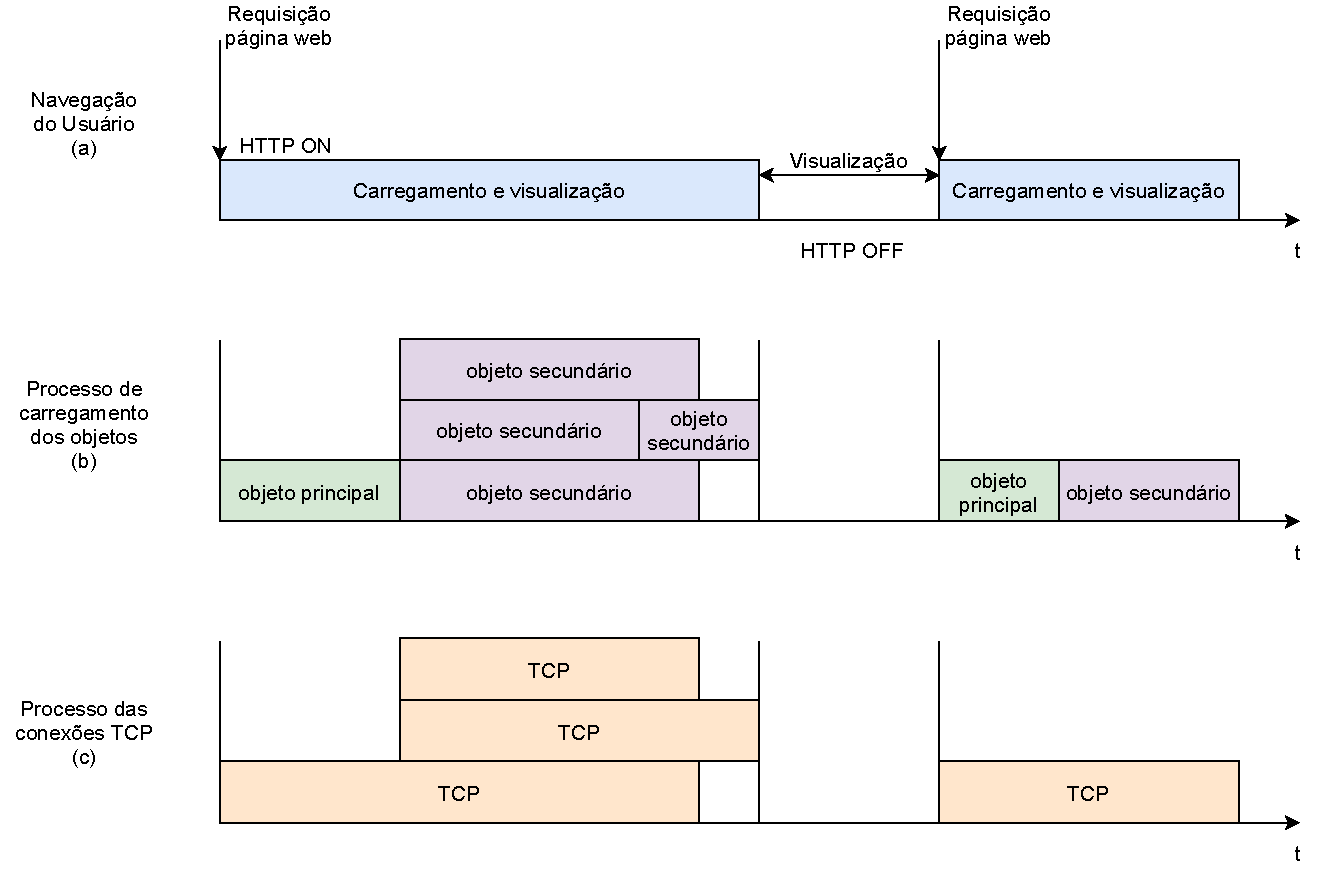
\includegraphics[scale=0.7]{textuais/http-process.pdf}
	\caption[Processos HTTP]{Processos HTTP (Adaptado de \cite{Pries2012}).
		\label{fig:http-process}}
\end{figure}


Inicialmente, o usuário faz a requisição de uma página web, por meio de um cliente web, geralmente um navegador. Passa-se então a uma fase em que o usuário visualiza os itens enquanto eles estão sendo transferidos do servidor web para o cliente (HTTP ON). Ao término da transmissão (HTTP OFF), o usuário continua visualizando o conteúdo, até que realiza uma nova requisição para outros elementos web.

Do ponto de vista do processo de carregamento dos objetos, a requisição da página web se inicia com o objeto principal, seguido dos respectivos elementos secundários que compõe a página web. Por fim, sob a ótica do protocolo TCP, podem ser abertas sessões paralelas para acelerar as transferências dos diversos objetos secundários.

Este comportamento em rajadas é descrito em diversos trabalhos na literatura, confirmando ainda a propriedade de escala desse efeito, ou seja, o comportamento se mantêm em um curto ou longo intervalo de análise, o que é denominado auto-similaridade (\textit{self-similarity}) \cite{Crovella1997}.

Na literatura, este comportamento pode ser modelado sob diferentes perspectivas \cite{Cheng2013}: baseado na página (\textit{page-based}), baseado no comportamento (\textit{behavior-based}) e baseado na conexão (\textit{conection-based}).

Modelos baseados na página, se preocupam apenas com a estrutura da página, sem considerar aspectos como atrasos dos servidores ou latência das requisições. Já os modelos baseados em comportamento, consideram o tráfego como uma aplicação ON/OFF. Por fim, o modelo baseado em conexões, modela o comportamento do tráfego HTTP considerando as características das sessões TCP, tais como taxa de estabelecimento de conexões, tamanho das requisições e respostas, intervalo entre os objetos, dentre outros.

Em \cite{Cheng2013}, \citeauthoronline{Cheng2013} afirmam que o modelo baseado em conexões é a melhor alternativa. Por outro lado, o modelo utilizado por estes autores é baseado em medições realizadas no ano de 1997, e que já não correspondem a realidade da web atual.

\citeauthoronline{Pries2012} apresentam em \cite{Pries2012} um modelo baseado em comportamento que, além de considerar o tráfego como uma aplicação ON/OFF, também define um intervalo de leitura para o usuário. Além disso, os autores analisaram as característica da estrutura de 1 milhão de páginas web ranqueadas como as mais acessadas no mundo. A partir dessas características, um modelo que detalha o tamanho dos objetos principais, tamanho dos objetos secundários e tempo de leitura do usuário foi consolidado. Este modelo corrige os problemas do modelo baseado em conexões, citados pelos autores em \cite{Cheng2013}, enquanto se aproxima do modelo baseado em conexões, apresentando dados mais atualizados, coletados em meados do ano de 2010. 

Vale ressaltar que mesmo o modelo apresentado em \cite{Pries2012}, já apresenta uma defasagem de mais de 10 anos para a web atual. Contudo, não foram encontrados trabalhos com a mesma relevância e contemporaneidade que pudessem substituir o modelo proposto por \citeauthoronline{Pries2012}.

Acredita-se que essa lacuna de trabalhos foi ocasionada pela evolução do tráfego HTTP nos últimos anos. Passando de um tráfego caracterizado por transmissões de páginas web em rajadas, hoje temos um tráfego HTTP dominado pelo conteúdo de vídeo, que por sua vez é caracterizado por uma alta demanda de recursos da rede e fluxo contínuo de dados em uma dada taxa de transmissão. Somado a este fato, é possível identificar também um maior uso da rede em dispositivos móveis \cite{cisco-newsroom-vni-2017-2022} \cite{g1-2016}. Portanto, a relevância desse novo comportamento pode ser observada na lacuna de trabalhos avaliando apenas o trafego web clássico e a pluralidade de trabalhos que consideram a transmissão de vídeo e dispositivos móveis.

Apesar da abundância de trabalhos, percebe-se que existem muitas diferenças nas abordagens e focos das pesquisas, priorizando aspectos como a análise do funcionamento do \textit{streaming} de vídeo \cite{Ramos-munoz2014} \cite{Ragimova2019}, modelos baseados em dispositivos móveis \cite{Fang2016}, comportamento do usuário na navegação \cite{Tsompanidis2014} \cite{Zhao2013}, bem como nas estratégias para otimizar a transmissão do HTTP a partir do DASH (\textit{Dynamic Adaptive Streaming over HTTP}) \cite{Waldmann2017}. 

Considerando-se este contexto de diferentes abordagens e a necessidade de estabelecer um modelo para a transmissão de vídeo via HTTP no gerador de tráfego proposto, acredita-se que o modelo recomendado por \citeauthoronline{Navarro-Ortiz2020} em \cite{Navarro-Ortiz2020}, que tem como base os valores estabelecidos pelo YouTube e apresentados em \cite{youtube-recommendations}, seja o mais adequado neste momento, dada a relevância e extensão da pesquisa realizada por esses autores.


\subsection{AMBIENTES DE SIMULAÇÃO}

Geradores de tráfego ganham maior relevância quando estão integrados em ambientes de simulação, uma vez que podem se beneficiar do uso contínuo por parte da comunidade de pesquisadores, recebendo melhorias com o passar do tempo.

Existem muitas propostas de sistemas para simulações em Redes de Computadores. Em consonância com os objetivos do projeto, foi possível elencar quatro características desejáveis para a escolha do ambiente de simulação \cite{SaulodaMata2017}: 
\begin{itemize}
	\item \textbf{Código aberto (Open Source):} a maioria dos softwares de código aberto são gratuitos. Simuladores comerciais geralmente apresentam um alto custo pela licença de uso. Além disso, os softwares de código aberto permitem customizações e ajustes de acordo com a necessidade.
	\item \textbf{Modelos confiáveis:} o ambiente de simulação deve apresentar modelos confiáveis que asseguram a validade dos resultados.
	\item \textbf{Implementação eficiente:} para possibilitar a simulação de um grande número de cenários, o ambiente de simulação deve apresentar implementação moderna para fazer uso eficiente dos recursos de hardware.
	\item \textbf{Boa documentação:} um software bem documentado é essencial para facilitar o uso, customizações e contribuições da comunidade de usuários.
\end{itemize}

Considerando as características elencadas acima, o ambiente de simulação Network Simulator 3 (ns-3) \cite{ns3-2021} se destaca por cumprir todos os requisitos.

O ns-3 é um simulador de redes do tipo \textit{discrete-event}, desenvolvido com o objetivo de atender demandas educacionais e de pesquisa. É um programa gratuito, distribuído sob a licença GNU GPLv2, publicamente disponível no site dos desenvolvedores. É um simulador de propósito geral, ou seja, possibilita o estudo de diversos aspectos de uma rede. Com uma estrutura modular, o ns-3 permite que funcionalidades e melhorias sejam integradas ao seu núcleo por meio de módulos. O núcleo e os módulos do simulador são implementados na linguagem C++. A Figura \ref{fig:ns-3-organization} apresenta uma representação dessa estrutura modular. O núcleo (\textit{core}) do simulador é responsável por prover funcionalidades que são comuns a todos os tipos de redes, tais como, eventos, aritmética de tempo e variáveis aleatórias. O módulo de rede (\textit{network}) é responsável por implementar a estrutura dos pacotes. Logo acima, diversos módulos são posicionados com funcionalidades específicas, dentre eles, os módulos de aplicações onde se encontram os geradores de tráfego. O módulo \textit{helper} facilita o processo de construção dos \textit{scripts} de simulação. Estes \textit{scripts} podem ser escritos em C++ ou Python e especificam os parâmetros de simulação (topologia, interface aérea, tempo de simulação, etc). 

\begin{figure}
	\centering
	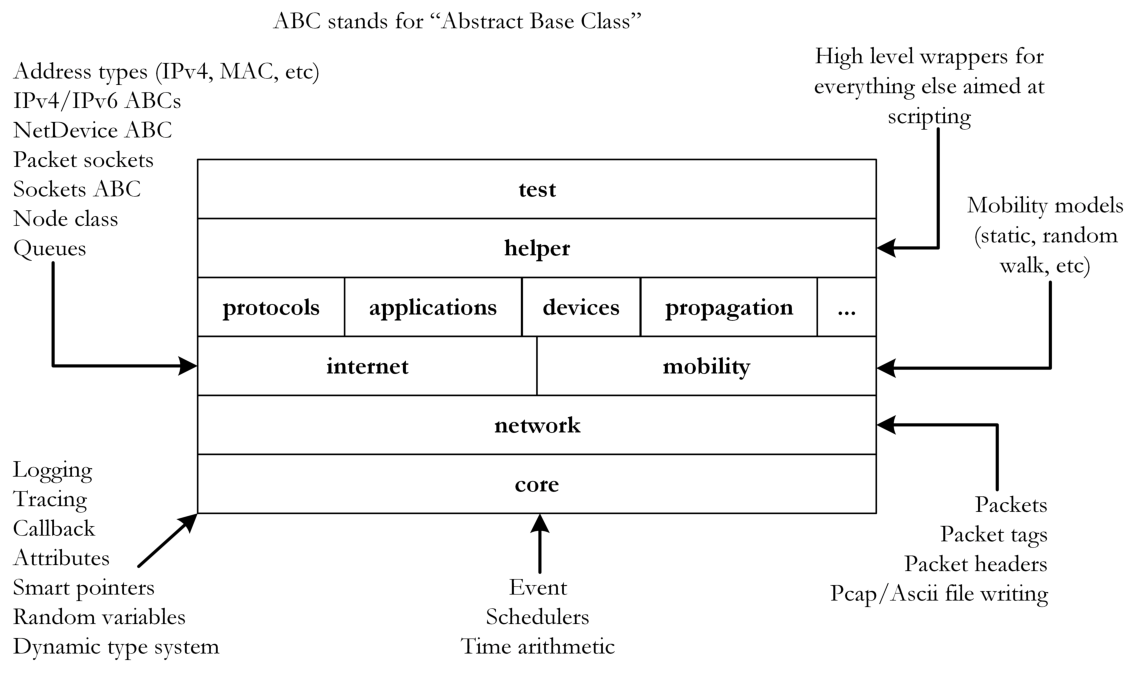
\includegraphics[scale=0.7]{textuais/ns-3-organization.pdf}
	\caption[Estrutura modular de organização do ns-3.]{Estrutura modular de organização do ns-3 (Adaptado de \cite{ns3-2021}).
		\label{fig:ns-3-organization}}
\end{figure}

No que concerne geradores de tráfego, o ns-3 apresenta, por padrão uma série de aplicações com características específicas endereçadas a diferentes propósitos dos usuários. Para o HTTP, o ambiente disponibiliza um módulo baseado em especificações publicadas em 2001 pelo 3GPP2 (3th Generation Partneship Project) publicadas em \cite{3GPP2-2001}. O módulo é interessante como guia de implementação para o gerador proposto neste projeto. Por outro lado, observa-se que o modelo matemático é baseado em dados com 20 anos de defasagem para a web atual.

Em \cite{Cheng2013}, \citeauthoronline{Cheng2013} apresentam uma proposta de módulo gerador de tráfego HTTP, baseado em conexões, para o ns-3. Este é o único trabalho encontrado com proposta similar ao projeto aqui delineado. Este módulo descrito em \cite{Cheng2013} apesar de apresentar uma implementação interessante, baseia-se em um modelo matemático com dados coletados em 1997 e não está integrado ao ns-3.

Dado o contexto atual da literatura do assunto, observa-se que exite um espaço de contribuição para um módulo com modelos matemáticos mais atualizados e funcionalidades que permitam o estudo do protocolo HTTP.
